\chapter{Sparse Matrix}

\section{Introduction}
A sparse matrix or sparse array is a matrix in which most of the elements are zero. The number  of zero-valued elements divided by total number of elements is called sparsity of the matrix. When storing and computing sparse matrix on device it is necessary to use the efficient algorithm and data structure. Because we can store sparse matrix in significantly in less storage.
\subsection{Storing}
A matrix is typically stored as a two dimensional or one dimensional but the length of one dimensional is equal to length of (row of matrix * length of column of matrix). For m x n matrix, we require (m * n * sizeof(float)) to store the matrix.\\
But in case, Sparse matrix we need 3 vector which is equal to (3*(size of non-zero element in matrix)* sizeof(float)).
\subsection{Storing formats}
\begin{itemize}
	\item Dictionary of keys (DOK)\\
		DOK consists of a dictionary that maps (row, column)-pairs to the value of the elements. Elements that are missing from the dictionary are taken to be zero. The format is good for incrementally constructing a sparse matrix in random order, but poor for iterating over non-zero values in lexicographical order. One typically constructs a matrix in this format and then converts to another more efficient format for processing. From \ref{txt:sparsematrixformat}
	\item List of lists (LIL)\\
	LIL stores one list per row, with each entry containing the column index and the value. Typically, these entries are kept sorted by column index for faster lookup. This is another format good for incremental matrix construction. From \ref{txt:sparsematrixformat}
	\item Coordinate list (COO)\\
	COO stores a list of (row, column, value) tuples. Ideally, the entries are sorted first by row index and then by column index, to improve random access times. This is another format that is good for incremental matrix construction. From \ref{txt:sparsematrixformat}
	\item Compressed sparse row (CSR, CRS or Yale format)\\
	 We explained in \ref{sec:csr} . From \ref{txt:CSR}
	\item Compressed sparse column (CSC or CCS)\\
	CSC is similar to CSR except that values are read first by column, a row index is stored for each value, and column pointers are stored. For example, CSC is (val, rowInd, colPtr), where val is an array of the (top-to-bottom, then left-to-right) non-zero values of the matrix; rowInd is the row indices corresponding to the values; and, colPtr is the list of val indexes where each column starts. From \ref{txt:sparsematrixformat}
\end{itemize}

\section{Compressed Row Storage (CRS)}
\label{sec:csr}
A sparse matrix or sparse array is a matrix in which most of the elements are zero. The number  of zero-valued elements divided by total number of elements is called sparsity of the matrix. When storing and computing sparse matrix on device it is necessary to use the efficient algorithm and data structure. Because we can store sparse matrix in significantly in less storage.\\
\textbf{Introduction}\\
The Compressed Row and Column Storage formats are the most general. They make absolutely no assumptions about the sparsity structure of the matrix and they don't store any unnecessary elements. On the other hand, they are not very efficient, needing an indirect addressing step for every single scalar operation in a matrix-vector product or preconditioned solve. From \ref{txt:CSR}\\
For CRS, we create 3 vectors and size of the vectors are length of non-zero elements of matrix. They are 
\begin{itemize}
	\item Non-zero elements of the matrix
	\item column number for non-zero elements of the matrix
	\item row number for non-zero elements of the matrix
\end{itemize}
\begin{center}
	\includegraphics[width=12cm]{../sparse.png} 
	\captionof{figure}{convert sparse matrix to CSR format}
	\label{img:csrfo}
\end{center}


The \texttt{val}  (\ref{img:csrfo}) represents the non-zero values of the matrix, read first by row left to right, then by column top to bottom. The \texttt{colind} represents the column index corresponding to the values. The \texttt{rowptr} represents the indexes belonging to a row, it contains an index per row corresponding to an index in the two other vectors. It is clear that all indexes from this starting index and to the starting index of the next row will belong to the given row. The last index is the number of rows plus one, so the algorithm doesn’t have to check if we’re at the last row.


In this project, We use Compressed sparse row (CSR, CRS or Yale format) for our implementation.

\section{Sparse matrix - vector multiplication}
\subsection{Introduction}
Matrix vector multiplication has been implemented in the API for all kinds of matrices. We will focus on CSR formatted sparse matrix vector multiplication. An example CSR formatting with indexes starting from 1 would be the matrix\\

The matrix vector product  using CRS format can be expressed in the usual way:
\begin{equation}
	y_i = \sum _{j=1}^{n} a_{ij}x_j \quad    i \in [1...m]
\end{equation}

\begin{center}
	$\begin{bmatrix}
	1&0&0&3\\
	0&2&4&6\\
	0&0&0&0\\
	0&5&0&0
\end{bmatrix}$
\captionof{figure}{sparse matrix}
\end{center}

which would be represented by the CSR format vectors:\\
val =[1 3 2 4 6 5]\\
val is the non zero element in sparse matrix Figure 3.1.\\
col =[1 4 2 3 4 2]\\
col is the column number of non zero element in sparse matrix Figure 3.1.\\
row =[1 3 6 6 7]\\
row is the row number of non zero element in sparse matrix Figure 3.1.\\


We can perform multiplications between a matrix and vector when number of columns of matrix equal number of rows of vector
\subsection{C++ implementation}
The C++ implementation is the most basic implementation. The idea is below\\
\begin{lstlisting}[language=C, caption=matrix vector multiplication in C++]
	for i < size of non_zero elements; i++
		result[row[i]] += non_zero[i] * vector[col[i]]
\end{lstlisting}
Listing 3.1, in each iteration of the for loop, the code computes the product of non-zero element of sparse matrix and position of column number of sparse matrix with same row number of vector element. And store the result on row number of non-zero element in sparse matrix.
It is better for time and space complexity. The time complexity of this algorithm is O(size of non-zero elements).
\subsection{OCCA implementation}
We implemented this algorithm in OKL as follow\\
\begin{lstlisting}[language=C, caption=matrix vector multiplication in OCCA]
	for i=0; i < #row of matrix; i++; @tile(16, @outer, @inner)
		for j = row[i]; j <row[i+1];j++
			result[i] += non_zero[j] * vector[col[j]]
\end{lstlisting}
Listing 3.2, In this algorithm, (\#row of matrix) is the number of row in matrix and row is a vector which save the number or non-zero elements in each row. For example, we have 2 non zero elements in row 0 then its row[0] = 0 and row[1] = 2.
The most challenging is the sparse matrix-vector multiplication v = Au. Due to the  restriction in accessing the OCCA memory it is not efficient to use the standard compressed storage data format.

This algorithm runs number of rows multiply number of non zero element in the row. It store the element in result vector and in every iteration, it compute the product of non zero element and column number of non zero element position of vector element.

\subsection{OCCA vs CPU}
\begin{center}
	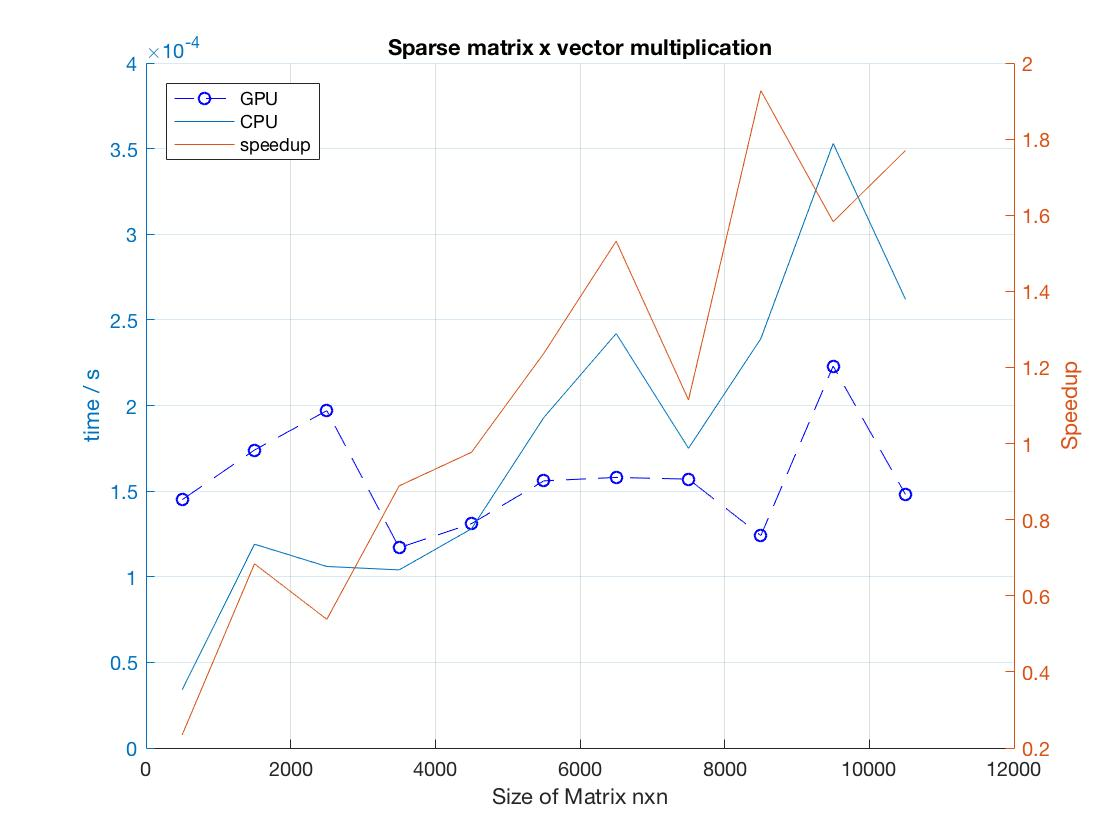
\includegraphics[width = 10cm]{Chapters/sparse_matrix_vector.jpg}
	\captionof{figure}{comparing OCCA vs CPU performance}
	\label{fig:comparisonSparse}
\end{center}
To test the performance of CPU and OCCA, we took a square sparse matrix and a vector. We save a sparse matrix in CSR format. Now we have 3 vectors, which stores non-zero elements of matrix, column number of non-zero elements in sparse matrix and row number of non-zero elements of the sparse matrix. For test cases, we use square sparse matrix. The dimension of the matrix starts from 500 by 500 to  10500 by 10500. The throughputs \ref{fig:comparisonSparse} of the CPU and OCCA as shown above. As we can see that the performance of CPU is better than OCCA, if dimension of the matrix is less than 4000. But dimension bigger than 4000, CPU performance is start fall down. And OCCA start perform better than CPU.


\section{Sparse matrix multiplication}
\subsection{Introduction}
Matrix multiplication has been implemented in the API for all kinds of matrices. We will focus on both CSR format sparse matrix multiplication. An example of CSR formatting the sparse matrix as follow\\

Let C is output matrix then mathematical formulation of the equation is described in (\ref{eq:sparsematrixmult})\\
\begin{equation}
\label{eq:sparsematrixmult}
	C_{ij}=a_{i1}b_{1j}+\cdots +a_{im}b_{mj}=\sum _{k=1}^{m}a_{ik}b_{kj}
\end{equation}
for i = 1, ..., n and j = 1, ..., p.\\
\begin{center}
	A= $\begin{bmatrix}
	1&0&0&3\\
	0&2&4&6\\
	0&0&0&0\\
	0&5&0&0
\end{bmatrix}$ B= $\begin{bmatrix}
	1&0&0&3\\
	0&2&4&6\\
	0&0&0&0\\
	0&5&0&0
\end{bmatrix}$
\captionof{figure}{A and B sparse matrix}
\end{center}

which would be represented by the vectors:\\
	A\_val =[1 3 2 4 6 5] \quad     B\_val =[1 3 2 4 6 5]\\
	A\_col =[1 4 2 3 4 2]  \quad    B\_col =[1 4 2 3 4 2]\\
	A\_row =[0 0 1 1 1 3]  \quad    B\_row =[0 0 1 1 1 3]\\


We can perform multiplications between a matrix and matrix when number of columns of matrix equal number of rows of another matrix.
\subsection{C++ implementation}
The C++ implementation pseudo code is below.
\begin{lstlisting}[language=C, caption=matrix multiplication in C++]
we use 2 vector for save the result of multiplication
int m =0;
for j < # of A non-zero elements; j++
	for k < # of B non-zero elements; k++
		check condition a_col[j] == b_row[k]
			check if the position of matrix already in array return position s
				result[s] += A_val[j]*B_val[k]
			otherwise
				result[m] = A_val[j]*B_val[k]
				position array[m] = A_row[j]* #number of column in matrix B
					 + B_col[k]
				m++
				
\end{lstlisting}
In CPU implementation, the j run from 0 to number of non-zero elements in A. Second loop k, start from 0 and end to number of the non-zero elements in B. It took j position of A\_col and compare with all the B\_row elements. Where A\_col is the column number of non-zero elements and B\_row is the row number of non-zero elements in matrix B. If we have same value on j position and k position than we have to multiply that elements and save it. After that we have to check if we already multiply and save the same row of matrix A and column of matrix B. If yes, then we have to add this in same element. If not, then we have to save result in new position of the result vector and position vector and increment the m. According to this procedure, we can save the memory because we do not need the matrix for saving the result.

\subsection{OCCA implementation}
The OCCA implementation in OKL:\\
\begin{lstlisting}[language=C, caption=matrix multiplication in OCCA]
for j < # of A non-zero elements; j++
	for o0 < # of B non-zero elements; o0++; outer
		for k = o0 k < o0+16; k++
			check condition a_col[j] == b_row[k]
					result[A_row[j]* # column in 
					matrix B + B_col[k]] = A_val[j]*B_val[k]
\end{lstlisting}
The OCCA uses the data parallelism in matrix multiplication. Except for the modified data structure for the sparse matrix storage the standard CRS matrix multiplication algorithm can be used with only minor modifications. In OKL, we just use for loops with an outer tag, which parallelised by threads (CPU) or work-groups (OCCA). We use inner tag in for-loops, which able to vectorized (CPU) or work concurrently (OCCA). The biggest problem of sparse matrix is result storage. As you can see that we are using the full length matrix for storing the result of two sparse matrix. The problem is OCCA do not define atomic operations clearly. All the working group work individually. It is not implemented till now.
\subsection{OCCA vs CPU}
\begin{center}
	\includegraphics[width = 12cm]{../matlab/sparse_matrix.jpg}
	\captionof{figure}{comparing OCCA vs CPU performance}
\end{center}
To test the performance of CPU and OCCA, we took two square sparse matrix. We save each sparse matrix in 3 vectors in CSR format. Now we have 6 vector for sparse matrices, which stores non-zero elements of matrix, column number of non-zero elements in sparse matrix and row number of non-zero elements of the sparse matrix. For test cases, we use square sparse matrices. The dimensions of the matrices start from 2000 by 2000 to  14000 by 14000. We use the semiology for plotting in Matlab. The throughputs of the CPU and OCCA as shown above. As we can see that the performance of CPU is better than OCCA, if dimension of the matrix is less than 10000. But dimension bigger than 10000, CPU performance is starting fall down. And OCCA start perform better than CPU. CPU rise too fast after 12000. Because when we increase the matrix size it also increase the non-zero elements in matrix.

\section{Sparse matrix - matrix addition \& subtraction}
\subsection{Introduction}
Sparse matrix addition or subtraction is not difficult. Firstly, we have to save both matrix in CSR formats.\\
Let C is output matrix then mathematical formulation of the equation is\\
\begin{equation}
	C_{ij}=a_{ij} \pm b_{ij}
\end{equation}

for i = 1, ..., n and j = 1, ..., p.\\
That is, the entry $C_{ij}$ is the sum or subtracion of the $i^{th}$ row and $j^{th}$ of A and the $i^{th}$ row and $j^{th}$ of B.\\
\begin{center}
	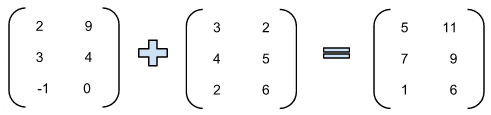
\includegraphics[width=10cm]{Chapters/matrix-matrix-addition} 
	\captionof{figure}{matrix addition}
\end{center}
	A\_val =[1 3 2 4 6 5] \quad     B\_val =[1 3 2 4 6 5]\\
	A\_col =[1 4 2 3 4 2]  \quad    B\_col =[1 4 2 3 4 2]\\
	A\_row =[0 0 1 1 1 3]  \quad    B\_row =[0 0 1 1 1 3]\\
	Normally, we have to add $j^{th}$ position of element of matrix A in $j^{th}$ position of element of matrix B and save it on $j^{th}$ position in result matrix.\\
	We have to be same dimensional matrices for addition or subtraction of matrices.
\subsection{CPU implementation}
CPU implementation addition (or subtraction) operation for sparse matrix with CSR format is described in the pseudocode:
\begin{lstlisting}[language=C, caption=matrix addition (or subtraction) in C++]
we have two vector of #non zero elements in A + #non zero elements in B

# copy A_non_zero elements to result
for i < #non zero elements in A; i++
	result[i] = A_non Zero [i]
	position[i] = A_row[i] * #number of column matrix A + A_col_number[i]
# copy B_non_zero elements to result
for i < #non zero elements in B;i++
	result[i+#non zero elements in A] = B_non Zero [i]
	position[i+#non zero elements in A] = B_row[i] * #number of column matrix B + B_col_number[i]
# checking if matrix a and matrix b have non zero element on same position
for i < #non zero elements in A + #non zero elements in B-1;i++
	for j < #non zero elements in A + #non zero elements in B;j++
		check condition i !=j && i<j
		check condition position[i] == position[j]
			result[i] += result[j]
			result[j] = 0;
			position[j] = 0;




\end{lstlisting}
As we can see, we have two vectors for save the output result and position. In result vector, we save the addition or subtraction of matrix A elements with matrix B elements. Position vector, we save the position of the result element. In this algorithm we are firstly save all the non zero element of matrix A and after we save all the non zero element of matrix B. As same as, we save position of all the non zero elements A and B in vector position. And in the end we just walk through the result vector and position vector. When we have duplicate element in vector position, we add that position element of result vector to the duplicate position element and make it zero and also remove element from the position vector make it zero.
\subsection{OCCA implementation}
The OCCA implementation for sparse matrix addition or subtraction pseudocode is below:
\begin{lstlisting}[language=C, caption=matrix addition (or subtraction) in OCCA]
we have two vector of #non zero elements in A + #non zero elements in B
for i < #non zero elements in A;i++;@tile(16, @outer, @inner)
	result[i] = A_non Zero [i]
	position[i] = A_row[i] * #number of column matrix A + A_col_number[i]
for i < #non zero elements in B;i++;@tile(16, @outer, @inner)
	result[i+#non zero elements in A] = B_non Zero [i]
	position[i+#non zero elements in A] = B_row[i] * #number of column matrix                                    B + B_col_number[i]
for o1 < #non zero elements in A + #non zero elements in B-17;o1++;@outer
	for o0 < #non zero elements in A + #non zero elements in B;o0++;@outer
		for i = o1; i < o1+16;i++;@inner
	for j = o0; j < o1+16;j++;@inner
		check condition i !=j && i<j
		check condition position[i] == position[j]
			result[i] += result[j]
			result[j] = 0;
			position[j] = 0;
\end{lstlisting}
Both plus and minus share the same code. I have only presented plus operation. While it's called matrix addition, it can work for all data types, but it only applies to the values. That is, in the sparse, we only store values for given coordinates, but we can still add a sparse matrix to a sparse matrix.\\
In OCCA implementation is similar to the CPU implementation, but in first two loops we add fourth clause tile in for-loop that indicating the type of parallelism to be take by the for-loop. After that next two loops we use the outer1 and outer0 in for-loops, which parallelised by threads (CPU) or working-groups (OCCA). Afterward we have for-loops with the inner tag, which able to be vectorized (CPU) or or work concurrently (OCCA). We have to check the condition i != j because it will add the same position value again and again. Now we have to check the duplicate element in position vector and add the same position result element. And make it zero in result vector and position vector. 
\subsection{OCCA vs CPU}
\begin{center}
	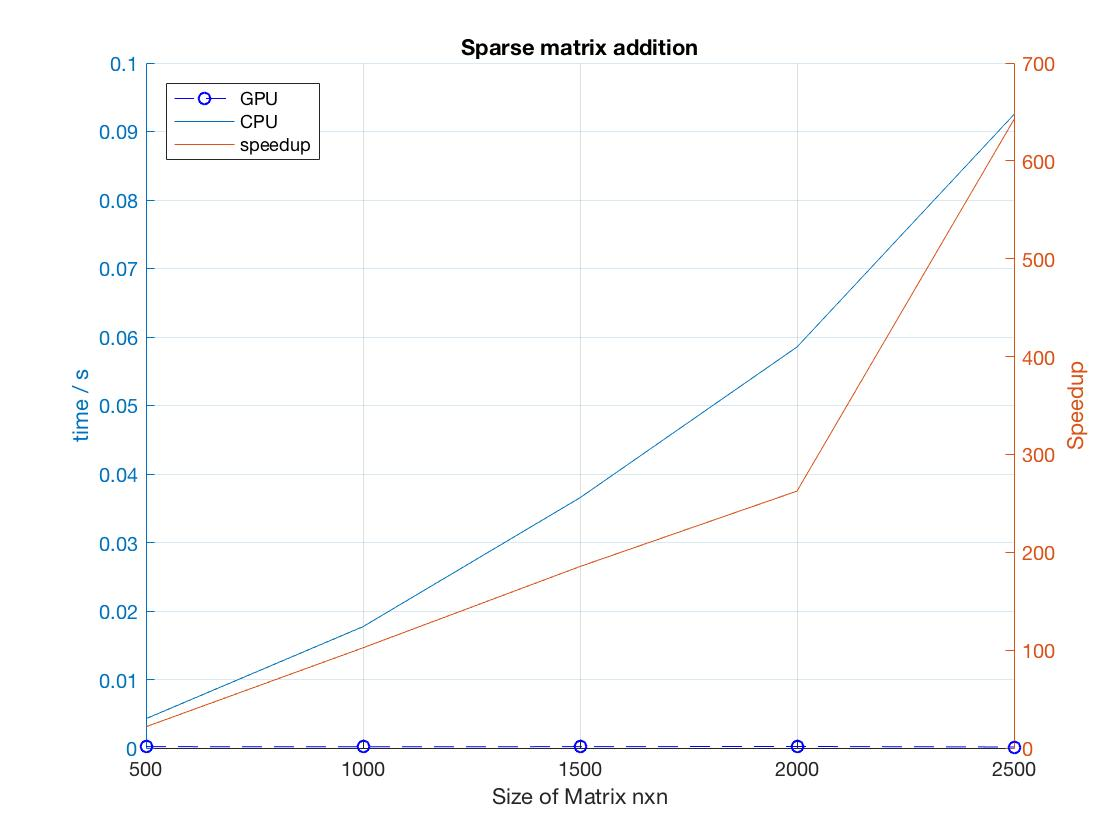
\includegraphics[width = 12cm]{Chapters/sparse_matrix_addition.jpg}
	\captionof{figure}{compare OCCA vs CPU performance }
\end{center}
As we can be see, the performance of CPU is not very good as expected. We use the two sparse matrices and convert it in the CSR format. The dimension of the matrix starts from 500 by 500 to  2500 by 2500. We use the semiology for plotting in Matlab. The throughputs of the CPU and OCCA as shown above. As we can see, the performance of OCCA is better than CPU, if we choose matrices size bigger.







